\documentclass{article}

\usepackage[utf8]{inputenc}

\usepackage{graphicx}
\usepackage{subcaption}
\usepackage{mathtools}
\usepackage{wrapfig}
\usepackage{graphicx}
\usepackage{subcaption}
\usepackage{mathtools}
\usepackage{wrapfig}
\usepackage{float}
\usepackage{gensymb}
\usepackage{caption}
\usepackage{geometry}
\usepackage{cite}

\DeclareMathOperator{\sech}{sech}
\DeclareMathOperator{\Tr}{Tr}

\usepackage{listings}
\usepackage{color}

\definecolor{codegreen}{rgb}{0,0.6,0}
\definecolor{codegray}{rgb}{0.5,0.5,0.5}
\definecolor{codepurple}{rgb}{0.58,0,0.82}
\definecolor{backcolour}{rgb}{0.95,0.95,0.92}
 
\lstdefinestyle{mystyle}{
    backgroundcolor=\color{backcolour},   
    commentstyle=\color{codegreen},
    keywordstyle=\color{magenta},
    numberstyle=\tiny\color{codegray},
    stringstyle=\color{codepurple},
    basicstyle=\footnotesize,
    breakatwhitespace=false,         
    breaklines=true,                 
    captionpos=b,                    
    keepspaces=true,                 
    numbers=left,                    
    numbersep=5pt,                  
    showspaces=false,                
    showstringspaces=false,
    showtabs=false,                  
    tabsize=2
}
 
\lstset{style=mystyle}




\makeatletter
\renewcommand\paragraph{\@startsection{paragraph}{4}{\z@}%
	{-2.5ex\@plus -1ex \@minus -.25ex}%
	{1.25ex \@plus .25ex}%
	{\normalfont\normalsize\bfseries}}
\makeatother
\setcounter{secnumdepth}{4} % how many sectioning levels to assign numbers to
\setcounter{tocdepth}{4}    % how many sectioning levels to show in ToC in preamble





\geometry
{
  %body={6.5in, 8.5in},
  left=1.0in,
  top=1.25in
}

\setlength{\parindent}{10ex}




%\begin{figure}[H]
%	\centering
%	\includegraphics[scale=0.2]{rhul_logo}
%\end{figure}

%questions for chris
%is there a paper for the creation of InterDyne that can be referenced, or is the webpage all there is?



\begin{document} 
\title{Defining the Semantics of Agent Based Modelling in Interdyne}
\author{Leo Carlos-Sandberg\\
Supervisor: Dr Christopher D. Clack} 
\maketitle 

\begin{abstract}
\noindent {\it This paper defines the semantics of agent based modelling within the Interdyne simulator. A converter has been created that links an agent based model step wise to a difference equation based language, this language is created in such a way that it is directly relatable to lambda calculus which can then be used as definition of the semantics of the agent based model.
%talk about this helping regulators 
}
\end{abstract}




\newpage
\newgeometry{top = 2cm}
\tableofcontents
{\textit{ }}
\restoregeometry
\newpage



%\begin{figure}[H]
%	\centering
%	\includegraphics[scale=0.5]{spin_on_lattice}
%	\caption{\it The two-dimensional Ising model lattice.}
%	\label{fig:spins_on_lattice_demo}
%\end{figure} 

%\begin{equation}
%E = -J\sum_{\langle i,j \rangle}^{N} s_{i}s_{j} - h \sum_{i = 1}^{N} s_{i}.
%\end{equation}

%\label{1d_code}

%~\cite{GouldBook} 
%~\ref{s_the_ising_model} 


\section{Introduction}
%introduce finicail markets
%Market Micrustrue, very research field at the cutting edge
%the need for interdyne, ergence in finciall markets is really investigated
%why i am doing what i am doing (need to example complex scientific predictions to econimsits etc)
%what i am doing (making a trasfeermation between DE and Agent based modeling)
%say that i am follwoing on from the work chris has done


%prove that the simulations are right
%Ability to provide confidence in the semantics of the system to economists and financial services industry practitioners
%Example ? difference equations (recurrence relations) ? provide a time-view, provides a way for economists to validate the description of the system (yes, we agree ? we understand these equations) 




\section{Background} 
This section explains the rational behind the creation of InterDyne by Clack~\cite{Chris_webPage}; InterDyne is bespoke simulation software designed to model emegernt behaviour within the financial markets. This research was inspired by the "Flash Crash" of 2010, this crash can be seen as a change in phase between a stable and unstable market; it has been shown that emergent behaviour in physical systems can lead to phase transitions and postulated that this could also be true within the financial markets~\cite{networkcastphorynature}. InterDyne hence exists to see if this flash crash and ones like it could be examples of this critical behaviour caused by emergence within the markets.     
This section will explain emergence within the financial markets, the approach taken to model these markets, examples of emergence within these models, a method to simulate these models and a detailed description of InterDyne.         


\subsection{Emergent Behaviour from Interaction Dynamics} 
%what is emegent behviour
%-microstystem to macrosystem
%-whats not emergence, can not claim indervidula elements contain the same properties as the system
%examples of emergence in other fields, physics chemistry bioligy etc
%-
%what are the interaction dynamics here and how do they lead to emergence
%why fincial markets? (they seems similar in strutre, different bodies interacting)
%fincial markets intteractitn dynamics (trading loans etc), focusing on trading
%why this interactions happen and why they are important (price impact etc)




Emergent behaviour describes properties of the macrosystem that are not inherent within the microsystem, in other words properties that emerge from the interaction of components of a system. A more formal definition is behaviour that can not be predicted through analysis of any single component of a system \cite{EB_systemofsystemsGLangford}




%https://www.researchgate.net/post/What_is_your_definition_of_emergent_properties
%https://arxiv.org/ftp/nlin/papers/0506/0506028.pdf
%https://www.researchgate.net/publication/265407712_THE_INTRINSIC_NATURE_OF_EMERGENCE
%https://phys.org/news/2015-04-complicated-self-organized-patterns-emergent-behavior.html

emegence leads to critical behviour and phase changes such as a flash crash
%http://www.cs.bris.ac.uk/home/dc/cliff_wtf_transcript_final.pdf
%http://nautil.us/issue/23/dominoes/why-the-flash-crash-really-matters



Emergent behaviour, described as behaviour that can not be predicted through analysis of any single component of a system [REF??? ]
%http://faculty.nps.edu/thuynh/Conference%20Proceedings%20Papers/Paper_14_Emergent%20Behavior%20in%20Systems%20of%20Systems.pdf
%describe these physical systems as systems of systems then describe the fincicial markets of systems of systems
, is a well known concept in scientific fields, such as physics chemistry and biology. A simple example of this phenomena is demonstrated in the game of life, see reference [REF],
%http://www.scholarpedia.org/article/Game_of_Life   
which shows the creation of large and complex patterns on a 2D grid from a few very simple rules. Real life examples include things such as, coupled oscillators [REF]
%[Wilberforce, Lionel Robert (1896). "On the vibrations of a loaded spiral spring". Philosophical Magazine. 38: 386?392]
and flocking dynamics [REF]. 
%flocking emergent behviour 
%http://ieeexplore.ieee.org/abstract/document/4200853
The high-level behaviour of note in these examples is generated from the interaction between components of these systems and would not be present with out the interactions. If a bird was to fly solo its trajectory would be relatively constant and no flocking would be observed as the need to avoid other birds and match their speed would not exist. Similarly if one of the coupled oscillators was removed then the remaining one would exhibit simple movement.\\  
The research that this paper is building on is primarily focussed on emergent behaviour with in the financial markets, it is relatively easy to see that given the huge complexity within the markets that emergent behaviour would occur. However noting that emergence occurs in relatively simple systems in real life, such as ????,
%example of rellativley simple system 
this research seeks to show that this is also the case within the financial markets.\\
Interactions in systems is just the passing of information from one entity to another, in the financial markets this is by electronic messages sent between the different players in the market, such as traders and exchanges. Nowadays most financial players operate algorithms in some capacity which will send and receive these messages, therefore the markets can be seen as a collection of interacting algorithms.   



























\subsubsection{Feedback Loops}
%this is a kind of emgent behifouvr
%what is a feedback loop
%how do they occur
%differnt kind of feedback loops (trades/loans)
%we are focusing on trading feeedback loops 
%static feeedbakc loops
%dynamic feedback loops
%static and dynamic analysis

A prominent form of emergence in the financial markets is feedback loops, this is where the input information to an entity is directly caused by its output information. The way in which the output information is transformed into the input information can be very simple, directly feeding back into the entity, or very complex going via an number of other entities before returning to its originator. Figure~\ref{fig:ex_feedback} demonstrates these two types of feedback loops with entity 1 having a direct feedback loop and a more complex feedback loop going through two other entities. 
\begin{figure}[H]
	\centering
	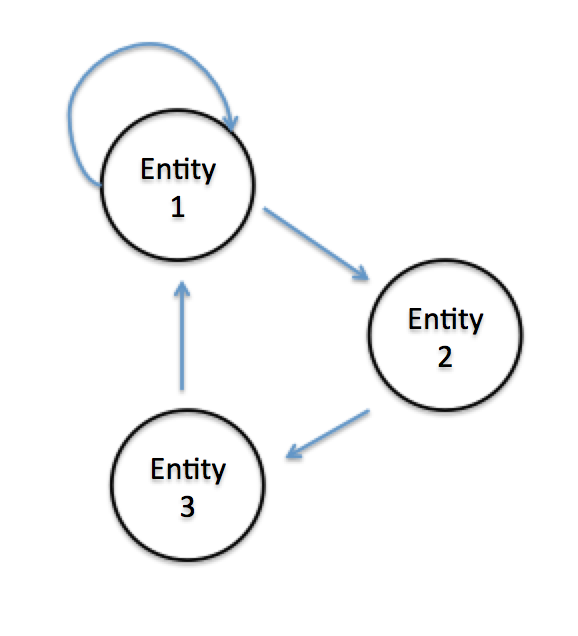
\includegraphics[scale=0.5]{feedback_loops_example}
	\caption{\it Feedback loops within a system of three interacting entities. Entity 1 has two feedback loops, one direct to its self, the other going through entity 2 and 3 before returning to entity 1.}
	\label{fig:ex_feedback}
\end{figure} 




 feedback oscillation in electronics [H. Barkhausen, Lehrbuch der Elektronen-R�hren und ihrer technischen Anwendungen: R�ckkopplung, Hirzel:Leipzig, 1935.].  An everyday example of undesirable behaviour arising from interaction arises when the loudspeaker output of an audio amplification system interacts with the microphone input; the interaction causes a feedback loop, resulting in a high-pitched oscillation.

19.1.2 Feedback loops
A good example of undesirable emergent behaviour in the financial markets is the creation of feedback loops, where a component system observes in its input some value that derives from its own output.  The process by which an output value is transformed into a derived input value may be complex and transitive (i.e. it may involve processing by one or more other component systems).
The description and classification of feedback loops is not straghtforward. Feedback loops may exist in a financial market ab initio, or may be created dynamically after the financial market has been operational for a period of time.  It is also possible for feedback loops to increase or decrease in size or effect, to split or merge, or to disappear.  Some feedback loops may have a benign effect (we call these stabilising loops) and some are malignant (destablilising loops).
In addition to categorising loops as either stablilising or destabilising, we identify whether they are static or dynamic.  For a given SoS, a static loop is one that always exists, with unchanging size and effect, and which could be detected by a straightforward static analysis of a formal description of the SoS.  Such loops may be intended or unintended.  By contrast a dynamic loop may be transient, may have changing size or effect, and might not be detectable via straightforward static analysis.  Dynamic loops may be highly unpredictable and difficult to detect, analyse and understand.

%\paragraph{Static Loops versus Dynamic Loops} 
%what is a static loop
%what is a dynamic loop
%why static loops are boring
%why dnamic loops are emegence 
%I am intrested in dynamic loops







A good example of complex interaction dynamics in the financial markets is the creation of feedback loops, where a component system observes in its input some value that derives from its own output.  For example, falling market prices can cause traders to sell (to prevent further loss) and this selling causes prices to fall further (which provokes further selling).
Some feedback loops may have a benign effect (we call these stabilising feedback loops) whereas others may be malignant (we call these destablilising feedback loops).  Control systems routinely use stabilising feedback loops to ensure an output signal stays close to a desired reference signal (See for example [Skogestad, Sigurd, and Ian Postlethwaite. Multivariable feedback control: analysis and design. Vol. 2. New York: Wiley, 2007, Zames, George. "On the input-output stability of time-varying nonlinear feedback systems part one: Conditions derived using concepts of loop gain, conicity, and positivity." IEEE transactions on automatic control 11.2 (1966): 228-238, and Horowitz, Isaac. "Fundamental theory of automatic linear feedback control systems." IRE Transactions on Automatic Control 4.3 (1959): 5-19.]).
The process by which an output value is transformed into an observed input value may be complex and transitive (i.e. it may involve intermediate processing by one or more other component systems); this is illustrated in Figure 19.1 below, where interactions between four components are depicted by directional arrows ? one direct feedback loop is depicted by an arrow from component 1 to itself, and one indirect feedback loop can be evinced by following the arrows from component 2 to component 3, to component 4, and back to component 2.  A practical example of a direct feedback loop would be a trading algorithm that issues orders to a stock exchange where the size and price of those orders is based on the previously issued order (or perhaps on a history of previously issued orders).  Alternatively, the size and price of an issued order may depend on the current size of the trader?s inventory ? when each order is executed at the exchange this will cause the trader?s inventory to be changed, and this will affect the next order issued. Notice how in these two examples the feedback loop does not exist in a single timestep but rather across timesteps ? the trader?s inventory is affected by orders filled in a previous time step, which are due to orders issued in a time step before that, and whose sizes were affected by the size of the trader?s inventory in a further previous time step.  The fact that a feedback loop extends across time steps does not make it less real (nor, potentially, less powerful) but it can make it more difficult to identify and to analyse.
LC- is using the term time step justified? Can you just say previously in time? As we havent introduced quantisied time yet, nor anything to do with time or how we will model it




Figure 19.1 - Four components, with one direct feedback loop and one indirect feedback loop.
When constructing a model of a financial market, the behaviour of the market components will be specified and initial conditions will be set.  In such a model, feedback loops may exist ab initio, and may potentially be discoverable by analysis of the specification and initial conditions.  We call this a static analysis of the specification, because it does not require the behaviour of the components to be traced (simulated) in time. Different kinds of static analysis may be required to identify different kinds of feedback loop ? for example, identification of a circular loan relationship between banks might require a different analysis to identification of a feedback effect on the calculation of order sizes for trading.
Alternatively, feedback loops might be created dynamically as a result of the changing behaviour of the components specified in the model (for example, a new loan relationship may create a feedback loop where there was none previously).  The role of the content of messages should not be underestimated, since coupling between components may for example depend upon the sizes of transactions and whether one component is buying or selling.  Similarly, dynamic coupling effects may involve several components, and feedback effects may depend upon repeated patterns of messages occurring between several components.  
To identify and understand such dynamically-created feedback loops requires analysis of the dynamic behaviour of the different components in the model ? for example, it requires the values of different functions and state variables to be traced from one time step to the next, and it may require inspection of the history of messages (including their data content) sent from one component to another.  We call this a dynamic analysis of the model. 
As part of dynamic analysis, we may also wish to investigate whether feedback loops increase or decrease in size or effect (that is, their effect on various ? typically high-level - properties of the model) and whether such feedback loops split, merge or disappear.
For a given model of a System of Systems, including its specification and initial conditions, we define a static feedback loop as one that always exists, with unchanging size and effect.  We expect that a static feedback loop is potentially discoverable by a static analysis of the model.  By contrast we define a dynamic feedback loop to be any feedback loop that is not static: i.e. it may be transient, may have changing size or effect, and might not be detectable via static analysis.  We expect that the identification of a dynamic feedback loop would require a dynamic analysis of the model, and we anticipate that dynamic feedback loops might be highly unpredictable and difficult to identify, analyse and understand.















\subsection{Approach to Modelling the Financial Markets}
%talk about work already done on this by other people
%looking at hft feedback loops (infrluenced by flash crash)
%market micrustrute 



%why I  am doing an example
	%this is the stuff we are actually looking at 
	%why look at the finical markets
%talking about what I am going to say in this section

from the book
Our focus is to explore emergent behaviour in the financial markets that arises from the dynamics of interaction between component systems, although the modelling and simulation technique that we use is applicable to other Systems of Systems.  We aim to assist economists, regulators, and financial services practitioners in understanding the complexity of such emergent behaviour; to model both simple and highly complex systems, to analyse and categorise emergent behaviour, to detect artefacts such as feedback loops, and to utilise modelling and simulation to predict the possible consequences of innovative practices (such as high-frequency trading) and regulatory interventions (such as transaction taxes).
Our initial interest in the financial markets derived from reading the reports of the staffs of the CFTC and the SEC into the ?Flash Crash? of May 6th 2010 [REF], coupled with observations from academics [REFS] and from industry practitioners [REFS].  We noticed that much of the approach and reasoning that was employed did not take into account the SoS nature of the financial markets; the issue of emergent behaviour was not discussed, and although the evidence presented in the formal CFTC/SEC report described several key feedback loops we felt that there was insufficient attention paid to the high-level market impact of low-level dynamic interaction, including these feedback loops. Our research therefore seeks to improve the conceptual understading of financial markets as a SoS with emergent behaviour arising from interaction dynamics.
	
\subsubsection{Fine-Grained Microstructure Approach to Financial Markets} 
%message passing
%order stacking
%order in which they are recived 
%delays between agents

%What is this approach
%why use this approach
%how this changes how we look at the fincial markets

from book
As we investigated the interaction dynamics involved in the Flash Crash, we realised that it would be necessary to model message-passing at a very fine-grained level.  For example, it would be necessary to model the timing of the arrival of limit orders at an exchange, because the sequence in which limit orders were processed by the exchange might support or defeat a feedback loop.  It would be necessary not only to model message-passing but also to run experiments to collect and observe the precise orderings of messages and their content. Furthermore, several reports [REFS] had mentioned the existence of communication delays and it was important to model the effects of increasing delays.  Thus, our task has been to model market microstructure [REF] in great detail

\subsubsection{Discrete Time}
%what is discrete time
%ns days months etc
%not event time
%why this occurs in fincial marekts

 
%this leads to discete time
%what is discrete time
%why this is good for us
Market Microsture 

Therefore, market microstructure describes financial markets both in terms of individual optimization problems and statistic ensembles of ?zero-intelligent? agents. Complicated global phenomena emerge as a result of the local interactions between many heterogeneous agents when the system throughput becomes sufficiently large.

from the book
When viewed in ?human time?, the financial markets appear to operate in continuous time. However, at a very fine-grained level of detail all computer operations are effected in discrete time dictated by the change in voltage of a system clock (a chip that emits an extremely precise square-wave oscillating voltage).  The passing of messages between two component systems of a financial market is a communication between two discrete-time systems linked by a transmission system; the transmission system itself would comprise a sequence of cables and intermediary devices, where the intermediary devices are typically operating in discrete time yet the cables (and the transmission delays introduced by the lengths of those cables) do not operate in discrete time.  Yet despite the continuous-time nature of some parts of the transmission system, a message will only be received by a computer at a discrete time determine by the receiving computer?s system clock (a message arriving earlier will not be processed until the next triggering edge of the clock voltage).
A challenge in modelling the interaction behaviour of financial markets is the linking of the extremely fast behaviour of discrete-time computers (and the automated trading and matching algorithms that they run) with the comparatively slow human observation of market behaviour.  
Another view of the markets that can be taken is an exceptionally large grain approach, where instead of looking at the markets in incredibly small time steps you instead look at larg ones, such as days, weeks, months or even years. Though this is not the approach taken in our research it will also lead to discrete time, where each time tick could be a new day. This approach could be used when investigating stock protifolies which are only rebalanced rarely. 

\subsection{Example}
%examples of real world feedbakc loops

Day and Huang [Day, R. And Huang, W., ?Bulls, Bears and Market Sheep?, Jourmal of Economic Behaviour and Organisation, 1990] for example have demonstrated how interactions between two simple but different trading strategies and a market-maker can cause complex emergent features of stock market prices such as alternating periods of rising (?bull market?) and falling (?bear market?) with sudden switching between the two at irregular intervals. Further, Lyons [Lyons, R.K. ?A Simultaneous Trade Model of the Foreign Exchange Hot Potato?, Journal of International Economics 42 (1997) 275?298] has shown how a feedback loop can emerge between foreign exchange dealers, causing them to repeatedly transfer inventory between themselves.  Yet these are simple models of interaction.  Our aim is to develop a framework for modelling and analysing more complex emergent behaviour that arises from the dynamics of interaction, and in the context of our case study to analyse behaviour that may increase risk to the stability of the financial markets.

\subsubsection{Hot Potato} 
%what is hot potato
%fx market

%this is a dynamic feedback loop
%how is it caused 
%when has it happened 

%what is a hft (probably need a subsectuion on this)
	%how do they work
	%what do they do
	%market makers
	%inventory limits
	%why do simple versions of them still work

To understand the hot potato effect one must first know that High Frequency Traders have strict inventory limits and that when these limits are passed they are said to be in a ``panic state''. During a panic state the traders will issue large sell market orders to reduce their inventories back into their ideal trading regions. A High Frequency Trader can go into a panic state when it unintentionally buys more inventory then intended, which can happen due to information delays in the confirmation of purchases. It is thought that in the flash crash High Frequency Trades panicked when buying from a mutual fund who issued an unusually large sell order. Once one High Frequency Trader has panicked its now sold inventory can be bought by another trader who, again because of information delay, surpass their inventory limits and in turn panics. This processes can continue indefinitely depending on the system and is known as the hot potato effect as the inventory is constantly passed around and not retained by an one trader~\cite{Elias_Paper}. This feedback effect has been shown, in the InterDyne simulator, to create instabilities in market prices and even lead to crashes~\cite{DynamicCoupling_Chris}.   

\subsubsection{Flash Crash}
%lob version of hot potato
 
%what is the flash crash
%when have they happned 
%other theories to why they happen?
%what we think causes them
	%emergence from feedback loops in hfts
%why they are important
A flash crash is defined as a quick drop and then recovery in securities prices, with the most infamous  crash occurring on the 6th of May 2010 and lasting for around 20 minutes in which time almost one trillion dollars of market value was lost~\cite{Vikram_Paper}.\\
There is no consensus on the exact cause of the flash crash, however a number of theories exist. The theory that InterDyne models is that the flash crash was caused by an interaction effect between High Frequency Trader Market Makers, known as the hot potato effect~\cite{Elias_Paper}. 

\subsection{Agent Based Modelling}
%modeligng techinques, no model is right but some are useful 
%what is agent based modelign
%why was it chosen
%what are its benifits for this
%what are its down sides

%what is agent based modleing
%http://ieeexplore.ieee.org/abstract/document/5679168/


\subsubsection{Benefits} 
%it has denifits and downsides
%why it is used for this
%its ebnfits
	%computation speed
	%ease of thinking
	%store messages
\paragraph{Tracking Messages} 
\paragraph{Conceptually Easy to Understand} 
%look at the notes for chris course for more reasons

\subsection{InterDyne} 
%this is what has been made
%how it works
%what has it been used for already

%what is interdyne
%how does it work
%what do we want it to show

InterDyne is a simulator designed to look at interaction dynamics, these dynamics have been with in the financial sector but can in theory be any interacting system. 
This is an agent based simulator, this means that each component of an interacting system can be expressed as an agent, in the case of a financial system agents could be individual traders. Interactions between the agents can then be defined, these could be messages sent between a trader and an exchange for placing an order. 
Once the simulator is set up in this way it can run through steps, at each step the interactions between the agents are passed and each agents response to the interaction is processed, these steps can represent discrete time.   
InterDyne adds no direct mechanism that would force the system as a whole to exhibit any specific behaviour, any emergent behaviour experienced by the system is a result of the interaction dynamics only.\\ 
A more complete way of labelling InterDyne would be as; a simulator used to investigate interaction dynamics and feedback effects in non-smooth complex systems~\cite{Chris_webPage}.





from book 
Interdyne is a simulator that is designed to allow for exploration of interaction dynamics and feedback effects in non-smooth complex systems, though this is a general purpose simulator that can be used in a variety of fields its setup makes it especially sorted to modelling the financial system that has been described above.  Below the aspects of Interdyne will be explained showing how it satisfies the criteria needed to model the finical markets. 
Like other agent-based models InterDyne operates in discrete-time, this discrete-time can be left without a proper definition in terms of real time, this is normally done in experiments that are interested purely in general behaviour of a system. Though real time mapping is easily achievable by simply taking the smallest time step that will need to be used with in a simulation and then mapping all time steps as a integer multiple of it.  
Being an agent-based model InterDyne allows communication between agents as the only form of interaction. This communication can be done in a one-to-one or one-to-many format, allowing for agents to send out broadcast messages which can be read by all other agents or send private correspondents that can only be seen by one other agent. Both of these messaging types are needed in modelling the markets, for example an exchange would send out a broadcast message to all members updating them on the order book, where as a trader would send a private message to a exchange when they want to place a order. 
To allow a full understanding and the precise use of these messages, a communication topology can be defined within InterDyne. This topology will defined the interaction paths between agents and as such which communication routes are possible and which are not. This topology takes the form of a directed graph (allowing on agent to trader with another but not vice versa) with the agents acting as the nodes and the communication paths acting as the edges. 
As with most real systems messages are not passed instantaneously and as such InterDyne supports the use of information delays, these delays are unique to each interaction path between agents, as defined in the communication topology.  These delays apply to any messages using these interaction paths, whether the message is defined as a one-to-one or a one-to-many.  





To allow InterDyne to model a system of systems and not just a flat system each agent can be modelled with differing levels of detail. This can take the form of having a simple agent generating outputs dependent on a statistical distribution, interacting with a trading algorithm, which contains a great amount of detail and complexity. An agent can also contain another InterDyne simulation as its internal structure, giving a true system of systems depth to the model.
The InterDyne simulator as a whole is built to be deterministic, meaning that any run of an experiment that contains the same inputs will always give the same output. This behaviour is very beneficial for analysis of low-level interactions that cause complex behaviour as it allows for a more detailed examination of the causal pathways that cause this behaviour. Though InterDyne is designed to be deterministic, non-determinism can be added to a simulation in two different ways. Either non-deterministic elements can be added directly to the agents (such as use of stochastic calculus to calculate some aspect of placing orders), or for an agent that receives multiple messages in one time step (such as an exchange receiving orders from a large number of traders) these messages can be sorted randomly (alternatively they can be sorted according to the senders identity).  This random sorting is in actuality pseudo-randomly, as for every run of the simulation the same random order will be reached, this can be changed to being truly random (or as much as a computer can allow) using a different seed for each run of the simulation.


\subsubsection{Harness} 
%used to connect the agents and monitor the interactions

\section {Description and analysis of the problem} 
%simulations in itnerduyne not fully excepted by exconimists


%this model is not fully excepted by econimists
%why this is so
%a method to fix this

\subsection{Why Agent Based Modelling is not enough}
%

%why agent based modeling is not perfect for being excepted
%one to many relationship
%an alternative differnce equations

\subsubsection{One-to-Many Problem}
\subsubsection{Semantics of the System} 
\subsubsection{Inverse Function Problem?} 

\subsection{Difference equations} 
%what are difference equations
%how do they work
%why are they more easily excepted

 \subsubsection{Benefits and Problems} 
 %other benfitis and down sides of them
 
 \subsubsection{Lack of Visualisation} 
%but they won?t be able to ?see? the emergent behaviour with running the simulator ?

\subsubsection{Optimisation Problems} 
% but generally we can?t directly ?run? these equations because for any reasonable-sized system there will be too much recomputation (we get the same problem with dynamic optimisation problems!)
%there are ways to cache intermediate results, but they ain?t pretty

\subsection{Two Views Approach} 
%My solutions, two view
%what is two views
%its benifits
%how it will solve the problem
%look at refrence in book chapter relating ABM to difference equations


from book
As can be seen in the previous sections there is no one perfect method for modelling the interaction dynamics and emergent behaviour with in the financial system. Due to the nature of this system it has been concluded that the two most useful models are difference equations and agent based models, however these two methods give very different views of the system making it impossible to be able to claim that one single method is more useful then the other in all cases. From this problem a natural question arises: is it possible to combine these two methods and hence reap the benefits that they both have, off setting the negatives of each other? The answer to this question we call the two-views approach, this is a way of combining both methods to tackle the same problem. The way in which we combine these two methods is to first define the problem using difference equations, allowing the benefits of this method to be used such as defining the semantics of the problem. Once the problem has been defined it is converted into an agent-based model using series of correctness preserving transformations. This allows the now agent-based version of this problem to still contain the same information that was present in its difference equation form, while now also now being able to be modelled with the benefits of the agent-based model.      
This method is specialised and a custom language for difference equations has been defined, that is an expansion of lambda calculus. This language has been defined in such a way that it can be used to express a problem so that the function of the agent-based model can still be fully utilised. The agent-based language that is used is designed to contain all the aspects need for expressing the financial markets: message passing, communication delays and interaction topology definition. We call this bespoke agent-based model Interdyne. 

\section{Converter} 
%how I will create the two views
%what the converter is meant to do


\subsection{New Language}
%first step is to create a language which can be used by a user to create a propram as difference equations
%language has to be simple enough that a non computer scientist/econimist can use, but must still be able to contain all the information required for the program
%programs wirtten in this language will be parsed into lexemes and then converted into a numeric type (?) which will be used to transfer this into lambda calcus and an ABM model

\subsubsection{Syntax/Grammer}
%what the new language looks like 
%what each bit means
%what is allowed to be written
%how to write certain things
%how is it user friendly
%why this was choosen, for example easier to convert to lambda calcualse 
\subsubsection{Parser}
%explain what the parser is and how it works, in preparing these files for transfermation
\subsubsection{Examples}
%examples on how to use the grammar
\paragraph{Simple Example}
%a very simple example on the use of the grammar
\paragraph{Complex Example}
%what I have actually done maybe?





\section{Conclusion}
\subsection{Further Work}

 
\section{Appendix}

\subsection{Appendix 1} %\label{Appendix_1}
%\lstinputlisting[language=C++]{AllCode_functions.cpp}


\addcontentsline{toc}{section}{References}
\bibliographystyle{unsrt}
\bibliography{MRes_Dissertation}







     
\end{document}










